\documentclass{article}

\usepackage{geometry}
 \geometry{
 a4paper,
 total={170mm,257mm},
 left=20mm,
 top=20mm
 }
\usepackage{float}
\usepackage{graphicx}
\usepackage{indentfirst}
\usepackage{hyperref}

\graphicspath{ {./images/} }
\renewcommand*\contentsname{Daftar Isi}
\renewcommand{\figurename}{Figur}
\renewcommand{\tablename}{Tabel}

\begin{document}
	\begin{titlepage}
		\begin{center}
			
			\null
			{
				\huge \bfseries Tugas Praktikum Pengembangan Perangkat Lunak}\\
			[1cm]
			{\LARGE Use Case KataHati}\\
			
			\vspace{2cm}
			
			\begin{figure}[H]
				\centering
				
\includegraphics[width=200px]{/HitamPutih.jpg}
			\end{figure}
			
			\vspace{3cm}
			
			{\Large 
				Disusun oleh Kelompok YapaYapaHuy} {\Large :\\
				\vspace{0.5cm}
				Ardacandra Subiantoro (18/427572/PA/18532)\\
				Chrystian (18/430257/PA/18770)\\
				Juandito Batara Kuncoro (18/427582/PA/18542)\\
			}
			
			
			\vspace{2cm}
			
			{\normalsize \bfseries
				PROGRAM STUDI S1 ILMU KOMPUTER\\
				DEPARTEMEN ILMU KOMPUTER DAN ELEKTRONIKA\\
				FAKULTAS MATEMATIKA DAN ILMU PENGETAHUAN ALAM\\
				UNIVERSITAS GADJAH MADA\\
				YOGYAKARTA\\
				\vspace{0.2cm}
				2020
			}
			
		\end{center}
	\end{titlepage}

	\newpage
	\pagenumbering{arabic}
	
	\section{Identifikasi}
	\subsection{Identifikasi Aktor}
	Aktor terlibat : \textbf{Mahasiswa, Tenaga Profesional,} \textbf{dan Administrator}
	\subsection{Identifikasi Use case dalam sistem}
	Use Case yang akan digambarkan dalam sistem :
	\begin{enumerate}
		\item Use case Mahasiswa Registrasi
		\item Use case Mahasiswa Login
		\item Use case Mahasiswa isi form
		\item Use case Mahasiswa mengajukan konsultasi
		\item Use case Mahasiswa membayar konsultasi
		\item Use case Mahasiswa melakukan konsultasi
		\item Use case Tenaga Profesional melakukan konsultasi
		\item Use case Admin membayar jasa tenaga profesional
	\end{enumerate}
	\subsection{Pengelompokan use case}
	Kelompok use case berdasarkan skenario :
	\begin{itemize}
		\item Use case \textbf{sebelum konsultasi} :  Mahasiswa registrasi, login, mengajukan konsultasi, membayar konsultasi
		\item Use case \textbf{saat konsultasi} :  Mahasiswa melakukan konsultasi, tenaga profesional melakukan konsultasi
		\item Use case \textbf{selesai konsultasi} :  Admin membayar jasa tenaga profesional
		\item \textbf{Opsional} : Mahasiswa isi form untuk menambah informasi tambaha pada saat konsultasi
	\end{itemize}
	
	\newpage
	\section{Use Case Diagram}
	\centering
	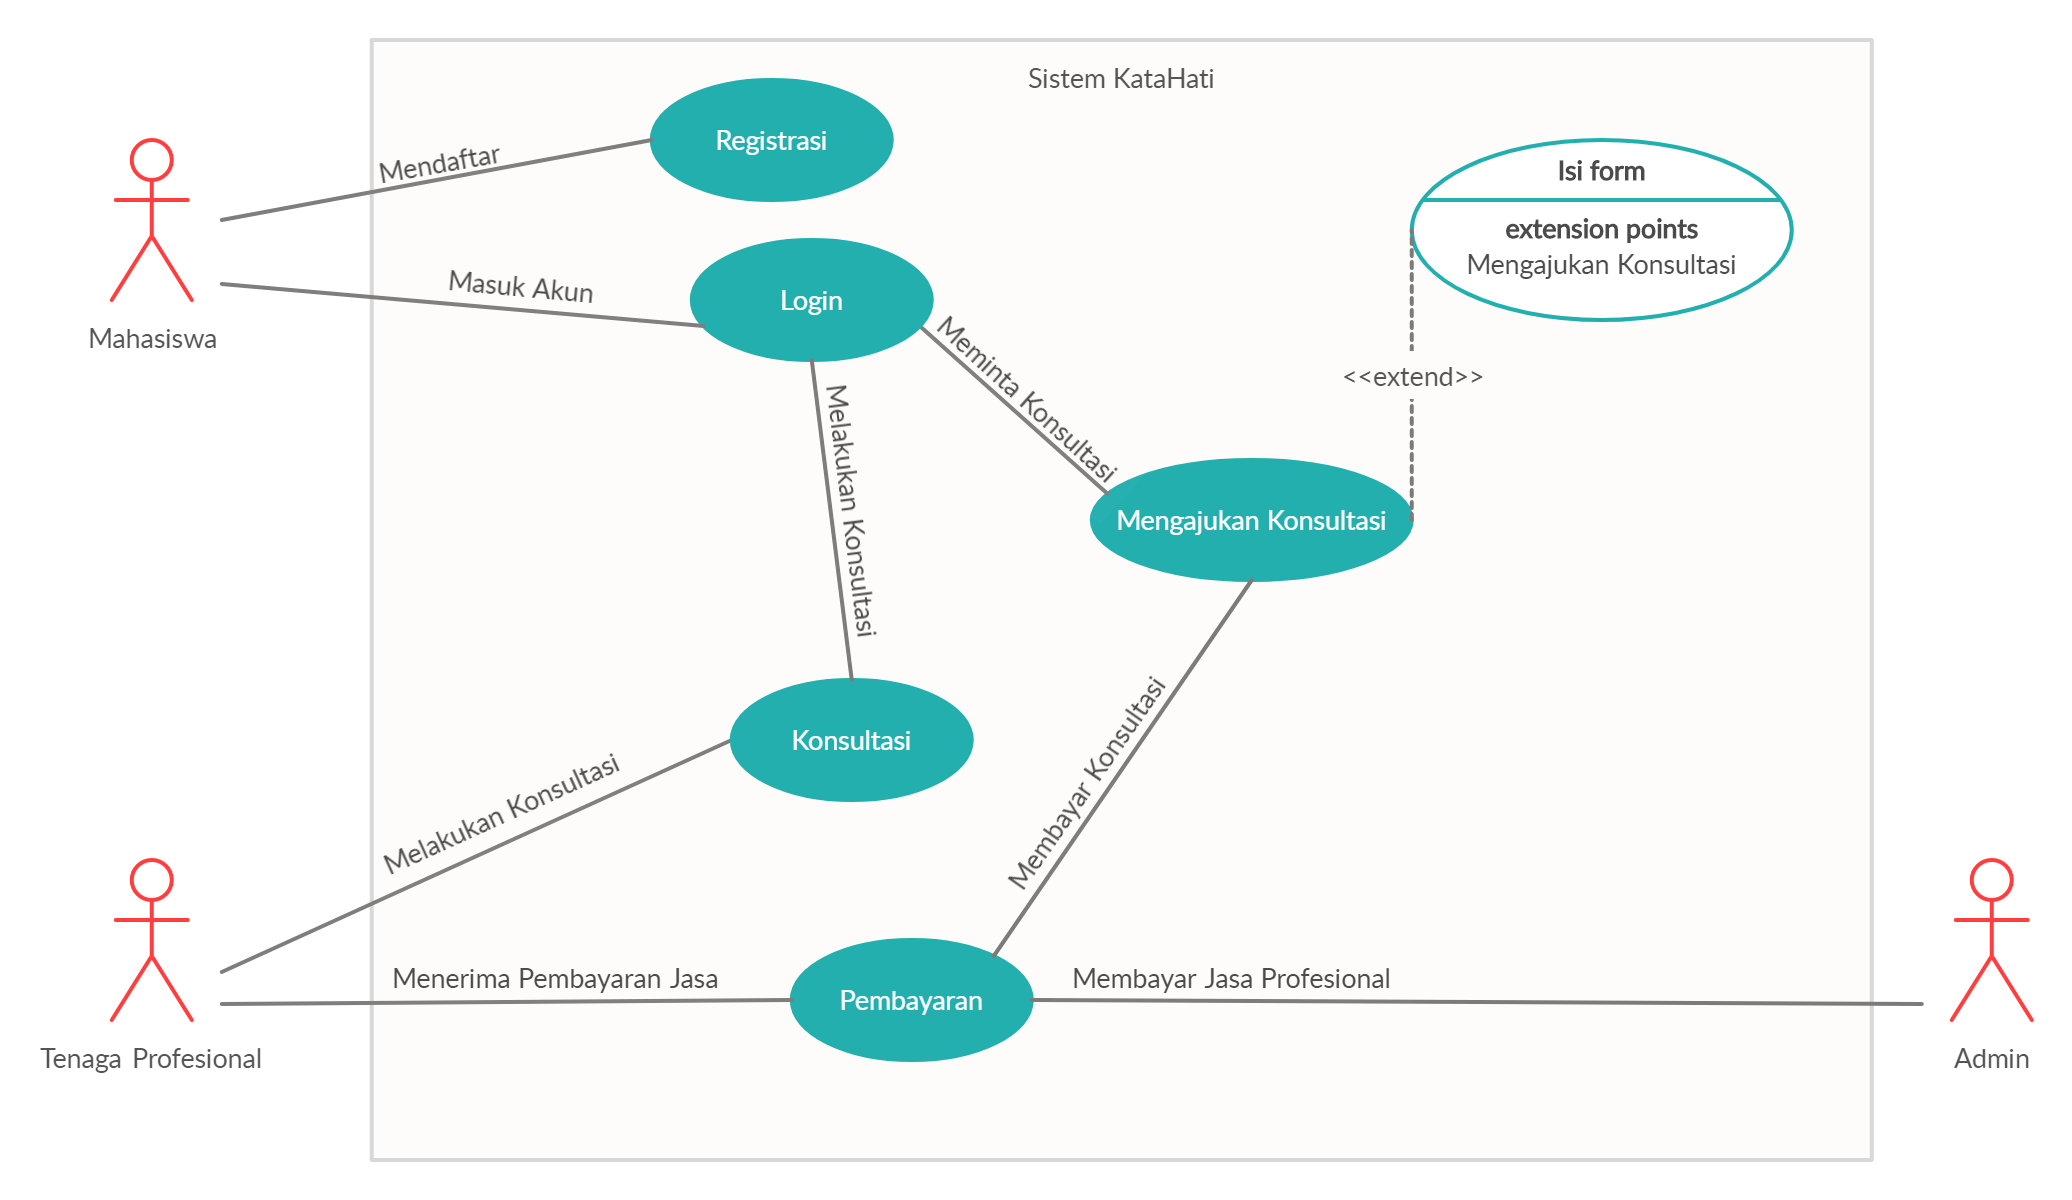
\includegraphics[width=160mm]{Use Case Kata Hati.png}
	\par
	
	
\end{document}